\let\negmedspace\undefined
\let\negthickspace\undefined
\documentclass[journal]{IEEEtran}
\usepackage[a5paper, margin=10mm, onecolumn]{geometry}
%\usepackage{lmodern} % Ensure lmodern is loaded for pdflatex
\usepackage{tfrupee} % Include tfrupee package

\setlength{\headheight}{1cm} % Set the height of the header box
\setlength{\headsep}{0mm}     % Set the distance between the header box and the top of the text

\usepackage{gvv-book}
\usepackage{gvv}
\usepackage{cite}
\usepackage{amsmath,amssymb,amsfonts,amsthm}
\usepackage{algorithmic}
\usepackage{graphicx}
\usepackage{textcomp}
\usepackage{xcolor}
\usepackage{txfonts}
\usepackage{listings}
\usepackage{enumitem}
\usepackage{mathtools}
\usepackage{gensymb}
\usepackage{comment}
\usepackage[breaklinks=true]{hyperref}
\usepackage{tkz-euclide} 
\usepackage{listings}
% \usepackage{gvv}                                        
\def\inputGnumericTable{}                                 
\usepackage[latin1]{inputenc}                                
\usepackage{color}                                            
\usepackage{array}                                            
\usepackage{longtable}                                       
\usepackage{calc}                                             
\usepackage{multirow}                                         
\usepackage{hhline}                                           
\usepackage{ifthen}                                           
\usepackage{lscape}
\usepackage{circuitikz}
\tikzstyle{block} = [rectangle, draw, fill=blue!20, 
    text width=4em, text centered, rounded corners, minimum height=3em]
\tikzstyle{sum} = [draw, fill=blue!10, circle, minimum size=1cm, node distance=1.5cm]
\tikzstyle{input} = [coordinate]
\tikzstyle{output} = [coordinate]


\begin{document}

\bibliographystyle{IEEEtran}
\vspace{3cm}

\title{4.3.37}
\author{EE25BTECH11001 - Aarush Dilawri}
\maketitle
% \newpage
% \bigskip
{\let\newpage\relax\maketitle}

\renewcommand{\thefigure}{\theenumi}
\renewcommand{\thetable}{\theenumi}
\setlength{\intextsep}{10pt} % Space between text and floats


\numberwithin{equation}{enumi}
\numberwithin{figure}{enumi}
\renewcommand{\thetable}{\theenumi}

\textbf{Question}:\\
Find the vector equation of the line passing through the point \brak{2,3,-5} and making equal angles with the coordinate axes.

\solution \\

Let the line be
\begin{align}
    \vec{x} = \vec{h} + \kappa\vec{m}
\end{align}
where $\vec{m}$ is the direction unit vector of the line ,  $\vec{h}$ is any given point on the line and $\lvert \kappa \rvert$ is the distance of $\vec{x}$ from $\vec{h}$ along the line.\\
Here,
\begin{align}
    \vec{h} = \myvec{2 \\ 3 \\ -5}
\end{align}
We are given that the line makes equal angles with the coordinate axes. Therefore,\\
\begin{align}
    \vec{m^T}e_1 = \vec{m^T}e_2 = \vec{m^T}e_3 = \lambda
\end{align}
where,
\begin{align}
    \vec{e_1} = \myvec{1 \\ 0 \\ 0},
    \vec{e_2} = \myvec{0 \\ 1 \\ 0},
    \vec{e_3} = \myvec{0 \\ 0 \\ 1}
\end{align}
from \brak{0.3},
\begin{align}
    \vec{m^T}\myvec{\vec{e_1} && \vec{e_2} && \vec{e_3}} = \lambda\myvec{1 && 1 && 1}\\
    \vec{m^T}\myvec{1 && 0 && 0 \\ 0 && 1 && 0 \\ 0 && 0 && 1} = \lambda\myvec{1 && 1 && 1}\\
    \vec{m^T}\vec{I} = \lambda\myvec{1 && 1 && 1}\\
    \vec{m^T} = \lambda\myvec{1 && 1 && 1}
\end{align}
Taking transpose on both sides,
\begin{align}
    \vec{m} = \myvec{\lambda \\ \lambda \\ \lambda}
\end{align}
Since,
\begin{align}
    \big\lVert \vec{m} \big\rVert = 1\\
    \lambda = \pm\frac{1}{\sqrt{3}}
\end{align}
Therefore the equation of the line is
\begin{align}
    \vec{x} = \myvec{2 \\ 3 \\ -5} + \kappa\myvec{\frac{1}{\sqrt{3}} \\ \frac{1}{\sqrt{3}} \\ \frac{1}{\sqrt{3}}} 
\end{align}

From the figure, it is clearly verified that the theoretical solution matches with the computational solution.
\begin{figure}[h!]
    \centering
    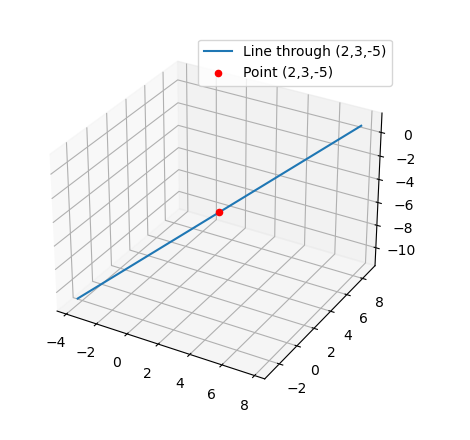
\includegraphics[height=0.5\textheight, keepaspectratio]{figs/fig.png}
    %\caption{Direction and Normal Vectors}
\end{figure}
\end{document}